\documentclass[a4paper]{article}


\usepackage{alphabeta} 
\usepackage{enumitem} 
\usepackage{mathtools}
\usepackage{amsmath, amssymb} 
\usepackage{amsthm}
\usepackage{cancel} 
\usepackage[margin=0.70in]{geometry} 
\geometry{left=2.9cm,right=3.0cm,top=2.1cm,bottom=2.3cm}	%the page geometry as defined, A4=210x297mm
\usepackage{graphicx}
\usepackage{wrapfig}
\usepackage{caption}
\usepackage{textcomp}
\usepackage{tabto}
\usepackage{layout}
\usepackage{bm}
\usepackage{minipage-marginpar}
\usepackage[dvipsnames]{xcolor}
\usepackage{hyperref}
\usepackage{dutchcal}
\usepackage{derivative}
\usepackage{esint}
%\usepackage{biblatex}
\usepackage{subcaption}
\usepackage{booktabs}\usepackage{derivative}
\usepackage[flushleft]{threeparttable}
\usepackage[capbesideposition=outside,capbesidesep=quad]{floatrow}
\usepackage{derivative}
\usepackage[thinc]{esdiff}
%%RENEW

\newtheorem{problem}{Άσκηση}
\newtheorem*{solution*}{Λύση}
\newtheorem{definition}{Ορισμός}[subsection]
\newtheorem{properties}{Ιδιότητες}[subsection]
\newtheorem{theorem}{Θεώρημα}[subsection]
\newtheorem{protash}{Πρόταση}[subsection]
\newtheorem{porisma}{Πόρισμα}[subsection]
\newtheorem{lemma}{Λήμμα}[subsection]
\newtheorem*{prooof}{Απόδειξη}
\newtheorem*{notes}{Παρατηρήσεις}
\newtheorem*{note}{Παρατήρηση}
\newtheorem*{app}{Εφαρμογή} 
\newtheorem*{example}{Παράδειγμα}
\newtheorem*{examples}{Παραδείγματα}


\newcommand\numberthis{\addtocounter{equation}{1}\tag{\theequation}}
%\renewcommand{\labelenumi}{\roman{enumi}}
\newcommand{\approxtext}[1]{\ensuremath{\stackrel{\text{#1}}{\approx}}}
\renewcommand{\figurename}{Εικόνα.}
\renewcommand{\tablename}{Πίνακας.}
%\renewcommand\refname{New References Header}
\renewcommand*\contentsname{Περιεχόμενα}
%\DeclareDerivative{\odv}{\mathrm{d}}


\begin{document}
\begin{titlepage}			%makes a title page. Remember to change the author, CID, username and group number to what is appropriate for you!
	\centering
	{\scshape\LARGE Εθνικό Μετσόβιο Πολυτεχνείο\par}
	{\scshape \LARGE Σ.Ε.Μ.Φ.Ε.\par}
	\vspace{1cm}
	{\huge\bfseries Ακτινοβολία Μέλανος Σώματος \par}
	\vspace{1cm}
	{\Large\itshape Θωμόπουλος Σπύρος\par}		%remember to change these!
	
	%		{\large Group \@group\unskip\strut\par}
	{\large A.M ge19042 \hfill \\ E-mail spyros.thomop@gmail.com \\}%ge19042@mail.ntua.gr\par		%remember to change these!
	\vspace{1cm}
	{\large Ημερμονηνία Παράδοσης 15/12/2021\par}
\end{titlepage}


\newpage 

\subsection*{Σκοπός}
Ο στόχος της εν λόγω πειραματικής άσκησης είναι η μελέτη της εξάρτησης της έντασης της ακτινοβολίας εκπομπής ενός μέλανος σώματος συναρτήσει του μήκου κύματος. Θα ελεγχθεί ο νόμος του Planck για την κατανομή της έντασης της ακτινοβολίας του μέλανος σώματος, όπως επίσης και οι "υπο-νόμοι" που περιέχονται σε αυτόν, δηλαδή ο νόμος της μετατόπισης του Wien και ο νόμος των Stefan-Boltzmann.

\subsection*{Θεωρητικά Στοιχεία}
Το σώμα που απορροφά όλη την προσπίπτουσα σε αυτό ηλεκτρομαγνητική ακτινοβολία ονομάζεται \textit{μέλαν σώμα.} Όταν ένα μέλαν σώμα βρίσκεται σε σταθερή θερμοκρασία Τ, ως αποτέλεσμα της θερμικής του ισορροπίας με το περιβάλλον (έστω και προσεγγιστικά), τότε εκπέμπει την λεγόμενη \textit{ακτινοβολία μέλανος σώματος}. \footnote{Ακόμη και τα σώματα που δεν είναι σε θερμική ισορροπία με το περιβάλλον τους εκπέμπουν ακτινοβολία, ένα μέρος της οποίας είναι της μορφής του μέλανος σώματος.}

Αν θεωρήσουμε τα εκπεμπόμενα φωτόνια ως ένα μποζονικό σύστημα, τότε γνωρίζουμε πως η πυκνότητα καταστάσεών του, δηλαδή ο αριθμός καταστάσεων που βρίσκεται στο διάστημα συχνοτήτων $(\omega,\omega+d\omega)$ είναι 
\begin{equation}\label{1}
f(\omega) = \frac{V\omega^2}{\pi^2c^3}
\end{equation}
Ακόμη, ο μέσος αριθμός κατάληψης των ενεργειακών στάθμεων για ένα τέτοιο σύστημα θα δίνεται από την κατανομή Bose-Einstein
\begin{equation}\label{2}
n_\omega^{(BE)} =  \frac{1}{e^{\beta \hbar\omega} -1 } 
\end{equation}
όπου $\beta = 1/kT$ και k η σταθερά Boltzman. Έτσι, η συνολική πυκνότητα ενέργειας (ενέργεια ανά μονάδα όγκου) για την εκπεμπόμενη ακτινοβολία ως προς την συχνότητα, είναι: 
\begin{equation}\label{3}
u(\omega)=\frac{\hbar\omega^3}{\pi^2c^3}\frac{1}{e^{\beta\hbar\omega} -1}=\frac{4h}{\lambda^3}\frac{1}{e^{hc/kT\lambda }-1}
\end{equation}
Η σχέση αυτή είναι η κατανομή του Planck αλλά για την πυκνότητα ενέργειας συναρτήσει της συχνότητας. Για να προκύψει  συναρτήσει του μήκους κύματος έχουμε
\begin{align*}\label{4}
u_\lambda d\lambda = -u_fdf  \Rightarrow u_\lambda =\frac{c}{\lambda^2}u_f = \frac{4hc}{\lambda^5}\frac{1}{e^{hc/kT\lambda }-1} \numberthis
\end{align*}
Άρα η ένταση της φασματικής κατανομής προκύπτει ως εξής 
\begin{equation*}\label{5}
I(\lambda,T) = u_\lambda (\lambda) \frac{c}{4} \Rightarrow 
\boxed{I(\lambda,T) =\frac{hc^2}{\lambda^5}\frac{1}{e^{hc/kT\lambda }-1}}	\numberthis \textit{"Κατανομή Planck για ένταση"}
\end{equation*}

Θέλοντας να βρούμε την τιμή του μήκους κύματος για την οποία η ένταση λαμβάνει μέγιστο απαιτούμε:
\begin{align*}\label{6}
\odv{I(\lambda,T)}{\lambda} &= 0 \Rightarrow 
\frac{-5}{\lambda^6}\frac{1}{e^{hc/kT\lambda }-1}+\frac{1}{\lambda^5}\frac{e^{hc/kT\lambda }}{(e^{hc/kT\lambda}-1)^2} \frac{hc}{kT\lambda^2} \Rightarrow \\ 
\frac{hc}{kT\lambda}\frac{1}{1-e^{-hc/kT\lambda}}&=5 
\xRightarrow{x:=hc/kT\lambda} 
x=5(1-e^{-x}) \xRightarrow{\text{Αριθμητική Επίλυση}} x\simeq 4.965 \Rightarrow \\ 
\lambda_{max} T &= \frac{hc}{4.965\cdot k} \Rightarrow  \boxed{\lambda_{max} T = 2.898\times 10^{-3} m\cdot K}\numberthis  \textit{ν. Wien}
\end{align*} 

Ολοκληρώνοντας την ένταση της σχέσης (\ref{4}) σε όλα τα δυνατά μήκη κύματος απο 0 έως $\infty$ παίρνουμε τον ρυθμό εκπομπής ακτινοβολούμενης ενέργειας ανά μονάδα επιφάνειας συναρτήσει της θερμοκρασίας

\begin{align*}\label{7}
I(T) = \int_0^{\infty} = I(\lambda,T)d\lambda \Rightarrow \cdots \Rightarrow \boxed{I(T)=\sigma T^4} \textit{ν. Stefan-Boltzmann} \numberthis
\end{align*}
όπου $\sigma = 5.675\times10^{-8}Wm^{-2}K^{-4}$ η σταθερά Stefan-Boltzmann.
\\
%\textcolor{red}{Μη ιδανικό μέλαν}
 Στην πραγματικότητα δεν υπάρχουν τέλεια μέλανα σώματα που απορροφούν όλη την προσπίπτουσα ενέργεια και γι' αυτό, η σωστή σχέση Stefan-Boltzmann είναι πολλαπλασιασμένη στο δεξί μέλος με μία σταθερά απορρόφησης $\alpha_\lambda = P_{\text{απορροφόυμενη}}/P_{\text{Προσπίπτουσα}}$.

\begin{wrapfigure}{r}{0.48\textwidth}
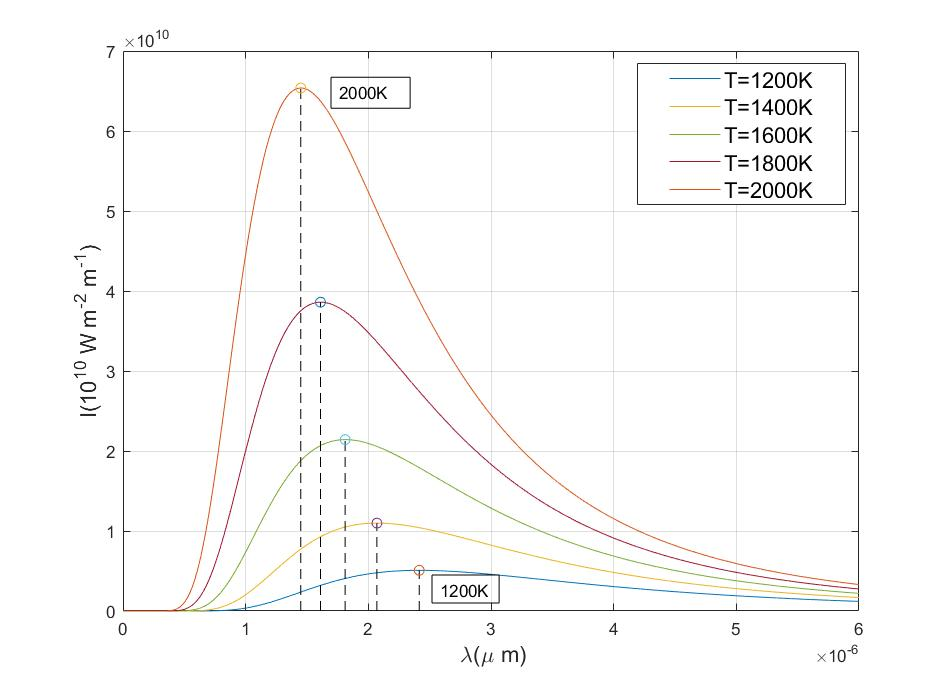
\includegraphics[width=1.45\linewidth]{planck_theory.jpg} 
\caption{Θεωρητικές Καμπύλες Κατανομής Planck	 }
\label{fig:wrapfig}
\end{wrapfigure}

Στην άκσηση αυτή θα προσεγγίσουμε το μέλαν σώμα με έναν λαμπτήρα πυρακτώσεως ο οποίος είναι κλεισμένος σε μία κοιλότητα. Η κοιλότητα αυτή έχει μία σχισμή από την οποία εκπέμπεται ακτινοβολία. Αυτή είναι η ακτινοβολία που μελετάμε και την θεωρούμε ως ακτινοβολία μέλανος σώματος. 

Μεταβάλλοντας την τάση που εφορμόζουμε στον λαμπτήρα, αλλάζει η θερμοκρασία του νήματος, άρα αλλάζουν και τα χαρακτηριστικά της εκπεμπόμενης ακτινοβολίας σύμφωνα με τους νόμους (\ref{6}) και (\ref{7}). Πιό συγκεκριμένα, αυξάνοντας την τάση θα αυξάνεται η θερμοκρασία και σύμφωνα με τον ν.Wien το μήκος κύματος στο οποίο εκπέμπεται η μέγιστη ένταση μειώνεται ενώ η συνολική εκπεμπόμενη ένταση αυξάνεται κατά τον νόμο των Stefan-Boltzmann.

Θα εξετάσουμε πειραμτικά τις εν λόγω αλλαγές στην εκπομπή ακτινοβολίας για διαφορετικές θερμοκρασίες.

\subsection*{Πειραματική Διάταξη}
Η πειραματική διάταξη περιλαμβάνει: 
\begin{itemize}
\item[$\rightarrow$] Πηγή ακτινοβολίας και μηχανισμό ευθυγράμμισής της με:
	\begin{itemize}
		\item[.] Λαμπτήρα πυρακτώσεως - προσομοιωτής της ακτινοβολίας μέλανος σώματος 
		\item[.] Διάταξη διέλευσης της φωτεινής δέσμης με σχισμές που δημιουργούν παράλληλη δέσμη
		\item[.] Φακοί ευθυγράμμισης της δέσμης
	\end{itemize}	
\item[$\rightarrow$] Φασματοφωτόμετρο πρίσματος που περιλαμβάνει: 
	\begin{itemize}
		\item[.] Βάση για το φασματοφωτόμετρο 
		\item[.] Πρίσμα γωνίας κορυφής $60^o$ για την ανάλυση-διασπορά της δέσμης ακτινοβολίας του λαμπτήρα
		\item[.] Φακοί εστίασης 
		\item[.] Οθόνη - Δίσκος ανοιγμάτων 
		\item[.] Αισθητήρας κίνησης για μέτρηση της γωνίας περιστροφής της οπτικής τράπεζας
		\item[.] Αισθητήρας φωτός
		\item[.] Περιστρεφόμενη τράπεζα, στην οποία τοποθετείται ένας οπτικός βραχίονας, το πρίσμα, ο δίσκος 				 				ανοιγμάτων και ο αισθητήρας ακτινοβολίας
	\end{itemize}
\item[$\rightarrow$] Σύστημα συλλογής πληροφοριών και ελέγχου της διάταξης, που έχει 
	\begin{itemize}
		\item[.] Διάταξη συλλογής δεδομένων από τους αισθητήρες φωτός που συνδέεται με τον Η/Υ
		\item[.] Ενισχυτής ισχύος, για την ενίσχυσης του σήματος που λαμβάνεται από τον αισθητήρα φωτός
		\item[.] Η/Υ με πρόγραμμα DataStudio
	\end{itemize}
\end{itemize}

\begin{wrapfigure}{r}{0.43\textwidth}
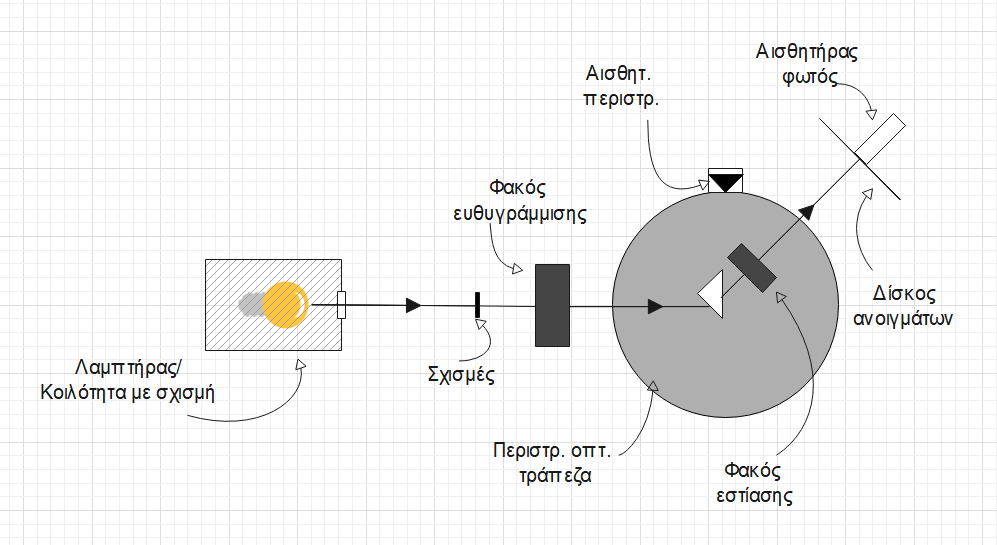
\includegraphics[width=1.3\linewidth]{setup.png} 
\caption{Διάταξη}
\label{fig:wrapfig}
\end{wrapfigure}
	
Ένα σχήμα της διάταξης με τα κυριότερα χαρακτηριστικά της φαίνεται στην Εικόνα 1.
%\begin{figure}[h!] 
%\centering 
%\caption{ }
%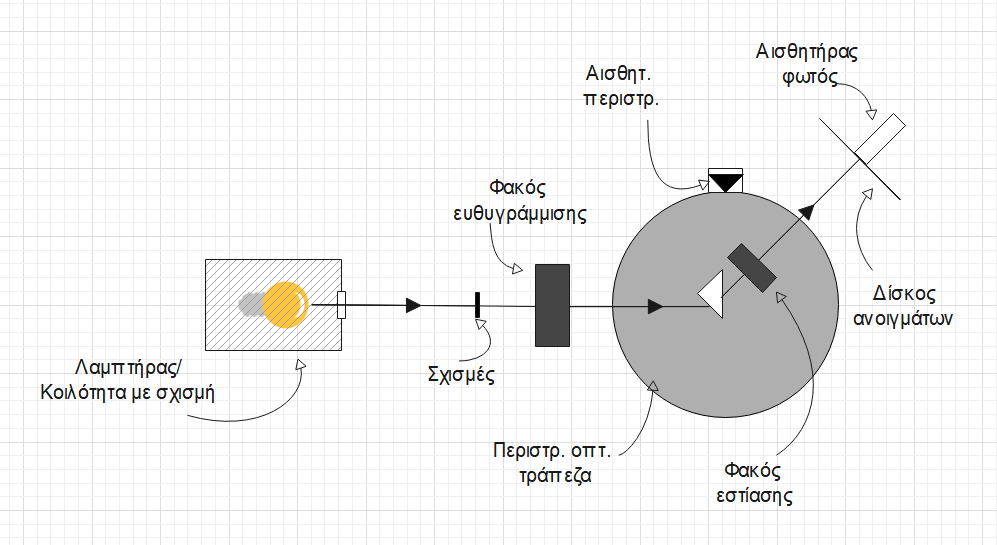
\includegraphics[scale=0.3]{setup.png}
%\end{figure}

Συνοπτικά, η μέθοδος είναι ότι αναλύουμε την ακτινοβολία του λαμπτήρα πυρακτώσεως που διέρχεται από την σχισμή με την βοήθεια του πρίσματος και τότε κάθε μήκος κύματος εκτρέπεται σε διαφορετική γωνία. Έπειτα, στρέφοντας την οπτική τράπεζα στην οποία είναι προσαρτημένος ο αισθητήρας μετράμε  την ένταση του φωτός συναρτήσει της γωνίας στροφής και κατ' επέκταση συναρτήσει του μήκους κύματος καθώς κάθε μήκος κύματος αντιστοιχεί σε διαφορετική γωνία.


\subsection*{Πειραματική Διαδικασία - Επεξεργασία Μετρήσεων}
Αρχικά θέτουμε σε λειτουργία την μονάδα συλλογής δεδομένων, τον ενισχυτή και τον Η/Υ στον οποίο θα λαμβάνουμε τις μετρήσεις. Μέσω του προγράμματος Blackbody.ds ορίζουμε την τάση στην λυχνία στα $V=5V$. Η κάθε τιμή της τάσης αντιστοιχεί σε διαφορετική θερμοκρασία. Αφού περιστρέψουμε τον βραχίονα στήρηξης του αισθητήρα στην μηδενική του θέση, διακόπτουμε την πορεία της ακτινοβολίας ώστε να μην φτάνει στον αισθητήρα. Πατώντας τωρα το κουμπί TARE, θέτουμε τον θόρυβο που λαμβάνει από το γύρω περιβάλλον ως το σημείο μηδέν των μετρήσεών μας. 

Ταυτόχρονα με τον μηδενισμό ξεκινάμε την καταγραφή των μετρήσεων (Κουμπί Start από το πρόγραμμα) και ταυτόχρονα περιστρέφουμε τον αισθητήρα μέχρι να έχουμε $\lambda\sim2500nm$ (Δεν ανιχνέυεται ένταση για μεγαλύτερο μήκος κύματος καθώς ο πυριτύαλος απ' τον οποίο είναι φτιαγμένο το πρίσμα δεν τα μεταδίδει). 

Επαναλαμβάνουμε τα παραπάνω βήματα μέχρι να πετύχουμε 5  αποδεκτές πειραματικές καμπύλες για τιμές της τάσης $V=5-9Volts$. Τα αποτελέσματα φαίνονται γραφικά στην Εικόνα 3.

\begin{figure}[h!]
\centering
\caption{Πειραματικά αποτελέσματα της κατανομής Planck }
\includegraphics[scale=0.4]{Planck_exper.jpg}
\end{figure}


Σε κάθε μία τιμή της τάσης αντιστοιχεί μια διαφορετική θερμοκρασία και γι' αυτό βλέπουμε αυτήν την μεταβολή στις παραπάνω καμπύλες, όπως άλλωστε περιμέναμε και θεωρητικά.  Η αντιστοίχιση αυτή καθώς και η τιμή του μήκους κύματος όπου λαμβάνεται μέγιστο έντασης φαίνεται στον Πίνακα Ι. Επίσης, εκεί φαίνεται το "Εμβαδόν" κάτω από την κάθε καμπύλη που είναι ανάλογο με την ολική ένταση της ακτινοβολίας και προκύπτει από το πρόγραμμα DataStudio. Οι υπόλοιπες στήλες του Πίνακα Ι χρησιμεύουν μετέπειτα για την επιβεβαίωση των νόμων Wien και Stefan-Boltzmann.

\begin{table}[h!]
\centering
\caption{ }
\begin{tabular}{r|r|r|r|r|r|r}
$V(Volts)$ & $T(K)$ & $\lambda_{max}(nm)$ & $1/T (10^{-4}K^{-1})$ & $\lambda_{max}T(10^{-3}m\cdot K)$ & Εμβδαδόν$(Wm^{-2})$ & $T^4(10^{13}K^4)$ \\ 
\hline\hline 
5&2028&1378&4.93& 2.79 &1336 &1.69\\
6&2169&1299&4.61& 2.82 &1760 &2.21\\
7&2300&1254&4.35& 2.88 &2200 &2.80\\
8&2419&1240&4.13& 2.99 &2688 &3.42\\
9&2530&1191&3.95& 3.01 &3275 &4.10\\
\end{tabular}
\end{table}

\subsubsection*{Νόμος Wien}

Απ' τον ν.Wien (\ref{6}) περιμένουμε ότι τα $\lambda_{max}$ και Τ θα είναι αντιστρόφως ανάλογα άρα τα $\lambda_{max}$ και $1/T$ θα είναι ανάλογα, δηλαδή θα σχετίζονται γραμμικά με ευθεία που περνά από την αρχή των αξόνων. Αν παραστήσουμε γραφικά τα εν λόγω μεγέθη προκύπτει το παρακάτω γράφημα για το οποίο προκύπτει η ευθεία ως μία πολύ καλή σχέση μεταξύ τους, καθώς η συσχέτισή τους (correlation) είναι: 
\footnote{Για να έχουμε μεγαλύτερη βεβαιότητα ότι ισχύει αυτή επιχειρηματολογία περί γραμμικότητας, ίσως να έπρεπε να έχουμε μεγαλύτερο αριθμό μετρήσεων, αλλά στην περίπτωσή μας που δεν ψάνχουμε τον νόμο, αλλά "κλέβοντας" λίγο προσπαθούμε απλώς να επιβεβαιώσουμε την γραμμικότητά του.}
\begin{align*}
correlation =\frac{ Cov[\lambda_{max},1/T]}{\sigma_{\lambda_{max}}\sigma_{1/T}} \simeq 0.80
\end{align*} 
όπου 
\begin{align*}
Cov[\lambda_{max},1/T] &= \sum_{i=1}^{N} \frac{((\lambda_{max})_i -\overline{\lambda_{max}})((1/				T)_i -\overline{(1/T)})}{N} = 0.0022    \\ 
\sigma_{\lambda_{max}} &=  \sqrt{\frac{\sum_{i=1}{N} ((\lambda_{max})_i -											\overline{\lambda{max}})^2   }{N(N-1)}} = 70.5    \\ 
\sigma_{1/T}           &=   \sqrt{\frac{\sum_{i=1}{N} ((T)_i -\overline{T})^2   }{N(N-1)}} = 3.9\times10^{-5}
\end{align*}



\begin{figure}[h!]
\centering 
\caption{ Γράφημα $\lambda_{max}$ - $1/T$.}
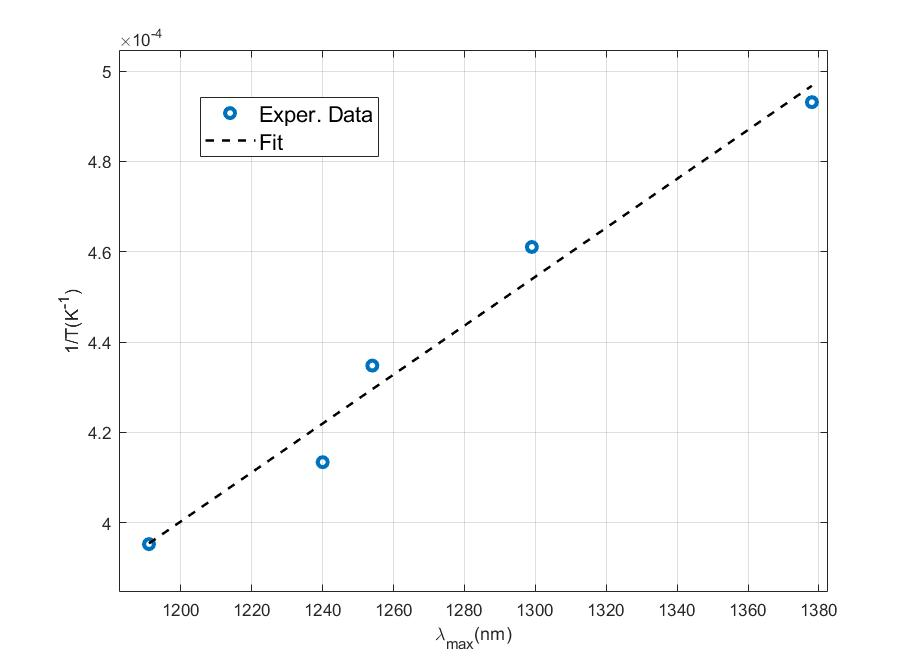
\includegraphics[scale=0.5]{wien_exper.jpg}
\end{figure}

Η μέση τιμή του γινομένου $\lambda_{max} T$ καθώς και το αντίστοιχο σφάλμα της είναι 
\begin{align*}
\overline{\lambda_{max}^T}      & =  \sum_{i=1}^{N} \frac{x_i}{N} = 2.90\times 10^{-3} m\cdot K   \\ 
\delta\lambda_{max} T &= \sqrt{\frac{\sum_{i=1}{N} ((\lambda_{max}T)_i -\overline{\lambda{max}T})^2   }{N(N-1)}}=0.05 \times10^{-3}m\cdot K 
\end{align*}

Άρα προκύπτει ότι 
\begin{align*}
\lambda_{max}T = (2.90\pm0.05)\times10^{-3} m\cdot K 
\end{align*}

Σε πρώτη φάση, η ισχύς του νόμου του Wien προκύπτει αρχικά από το ότι η συσχέτιση(correlation) των μεγεθών $\lambda_{max}$ και $1/T$ είναι κοντά στο 1, που σημαίνει πως έχουν γραμμική εξάρτηση. Ακόμη, παρατηρούμε πως το γινόμενο $\overline{\lambda_{max}} T$ είναι 
κοντά στην θεωρητικώς αναμενόμενη τιμή των $2.898\times10^{-3}m\dot K$ η οποία περιλαμβάνεται και στα όρια του σφάλματος της μέσης τιμή που έχει βρεθεί. Άρα μπορούμε να πούμε πως επιβεβαιώνεται ο ν.Wien.

\subsubsection*{Νόμος Stefan-Boltzmann}
Ομοίως με πριν, για την συσχέτιση των μεγεθών του "Εμβαδού" και του $T^4$ έχουμε ότι
\begin{align*}
correlation =\frac{ Cov[Area,T^4]}{\sigma_{Area}\sigma_{T^4}} \simeq 0.8
\end{align*}
Άρα επειδή είναι κοντά στο 1 η εξάρτησή τους είναι γραμμική (πιό σωστά έπρεπε να γράψω "ενδέχεται να είναι γραμμική" αλλά εδώ είναι κάπως σαν να την θεωρούμε εκ των προτέρων γραμμική) και προκύπτει η παρακάτω γραφική παράσταση από την μέθοδο των ελαχίστων τετραγώνων. 

\begin{figure}[h!]
\centering 
\caption{ Γράφημα "Εμβαδόν"-$T^4$}
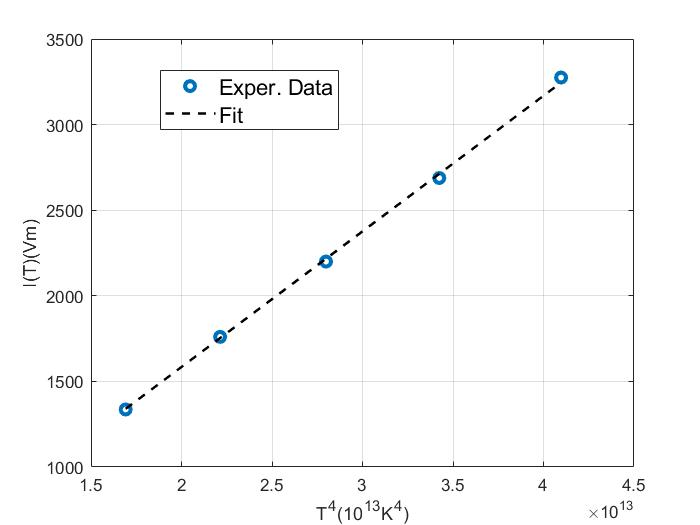
\includegraphics[scale=0.6]{stefan_exper.jpg}

\end{figure}
%Από την μέθοδο ελαχίστων τετραγώνων προκύπτει επίσης ότι η κλίση της ευθείας και το αντίστοιχο σφάλμα της είναι: 
%\begin{align*}
%B = (7.92\pm0.03)\times10^{-11}
%\end{align*}

Δεδομένου ότι το "Εμβαδό" δεν πρόκειται για την ολική ένταση της ακτινοβολίας, αλλά για την αντιστοιχία της σε κάποια τάση η οποία μετράται, δεν μπορεί να προκύψει η σταθερά $\sigma$ των  Stefan-Boltzmann.
 Ωστόσο, η επιβεβαίωση του νόμου είναι η αναλογία των μεγεθών $\text{"Εμβαδόν"}\sim T^4$ καθώς το εμβαδόν είναι ανάλογο της ολικής έντασης της ακτινοβολίας.


Όσο μειώνουμε την παρεχόμενη τάση, δηλαδή την θερμοκρασία του νήματος, προφανώς μειώνεται η ένταση του φάσματος που βλέπουμε. Ακόμη, η περιοχή του ιώδους γίνεται πιό αχνή από την περιοχή του ερυθρού και στις χαμηλότερες τάσεις σχεδόν δεν φαίνεται. Αυτό, διότι από την Εικόνα 3 (ν. Planck) βλέπουμε ότι το μέγιστο μήκος κύματος εκπομπής βρίσκεται στο υπέρυθρο άρα εγγύτερα στο ερυθρό απ' ότι στο ιώδες.




\subsection*{Συμπερσάσματα}
Συμπερασματικά, "επιβεβαιώνεται" ο νόμος του Planck καθώς έχουν "επιβεβαιωθεί" δύο απ' τις συνέπειές του, οι νόμοι Wien και Stefan-Boltzmann. "Επιβεβαιώνονται" σε εισαγωγικά, καθώς υπάρχουν κάποια σφάλματα λογικής κατά την επιχειρηματολογία, τα οποία στα πλαίσια της εν λόγω άσκηση ενδεχομένως να μην δύνανται να ξεπεραστούν και γι' αυτό αγνοούνται. Δηλαδή είναι σαν να θεωρείται εκ των προτέρων δεδομένη η γραμμική σχέση μεταξύ $\lambda_{max}-1/T$ και "Εμβαδόυ"-$T^4$. Προφανώς!, σε αυτή τη περίπτωση η συσχέτιση που βγαίνει $\simeq0.8$ ΔΕΝ! είναι και πολύ ισχυρό τεκμήριο για την γραμμικότητα απλώς χρησιμοποιείται ως μία \underline{παρα πολύ ασθενής ένδειξη} λόγω έλλειψης άλλης επιχειρηματολογίας.
\subsection*{Βιβλιογραφία}
\begin{itemize}
\item[.] Σημειώσεις του David Tong : http://www.damtp.cam.ac.uk/user/tong/teaching.html 
\item[.] https://en.wikipedia.org/wiki/Planck%27s_law 
\item[.]  ΣΤΑΤΙΣΤΙΚΗ ΦΥΣΙΚΗ, F.MANDL
\item[.] ΕΡΓΑΣΤΗΡΙΑΚΕΣ ΑΣΚΗΣΕΙς ΦΥΣΙΚΗΣ ΤΟΜΟΣ ΙΙ, ΣΥΛΛΟΓΙΚΟ
\end{itemize}
\end{document}